\documentclass{standalone}
\usepackage{tikz}
\usepackage{ctex,siunitx}
\setCJKmainfont{Noto Serif CJK SC}
\usepackage{tkz-euclide}
\usepackage{amsmath}
\usetikzlibrary{patterns, calc,3d}
\usetikzlibrary {decorations.pathmorphing,decorations.pathreplacing,decorations.shapes}
\tikzset{label style/.append style={font=\small}}
\begin{document}
\small
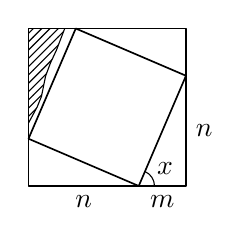
\begin{tikzpicture}[>=latex,scale=1.0]
  \tkzDefPoints{0/0/A,2/0/B,2/2/C,0/2/D}
  \tkzDefPointOnLine[pos=0.7](A,B)\tkzGetPoint{A'}
  \tkzDefPointOnLine[pos=0.7](B,C)\tkzGetPoint{B'}
  \tkzDefPointOnLine[pos=0.7](C,D)\tkzGetPoint{C'}
  \tkzDefPointOnLine[pos=0.77](C,D)\tkzGetPoint{C''}
  \tkzDefPointOnLine[pos=0.7](D,A)\tkzGetPoint{D'}
  \tkzDefPointOnLine[pos=0.6](D,A)\tkzGetPoint{D''}
  \begin{scope}
    \clip (0,0)rectangle(2,2);
    \draw[decorate,decoration={random steps,segment length=2mm,amplitude=1pt},pattern=north east lines](D'')--(C'')--(-0.2,2.2)--cycle;
  \end{scope}
  \tkzDrawPolygon[semithick](A,B,C,D)
  \tkzDrawPolygon[semithick](A',B',C',D')
  \tkzLabelLine[pos=0.5,below](A,A'){$n$}
  \tkzLabelLine[pos=0.5,below](A',B){$m$}
  \tkzLabelLine[pos=0.5,right](B,B'){$n$}
  \tkzMarkAngle[size=0.2](B,A',B')
  \tkzLabelAngle[pos=0.4](B,A',B'){$x$}
  
\end{tikzpicture}
\end{document}